\title{Week 1 Journal}
\author{Kevin Cardenas}

%\begin{document}
\maketitle

\section{Introduction and Goals for CS6000}

My name is Kevin Cardenas and I am a Captain in the US Air Force. I have the unique opportunity to be a full-time PhD student for my job as an active duty military member. I taught in the Department of Computer and Cyber Sciences at the USAF Academy for three years and will be able to go back to teaching after completing my PhD. The most challenging aspect of my PhD will be the fact that the Air Force only grants me three years to complete my degree. I chose to get a PhD in Computer Science so I could become a better asset for the USAF Academy and broaden my experience in the realm of Data Science. This will most likely add to the challenge of completing this degree in three years, but I like challenges. 

One of my primary goals for this course is to learn how to quickly sift through large volumes of articles/conference papers/journals/etc to find pertinent information relating to my area of research. A secondary goal for this course is to have a well defined research topic by the end of the semester. These two goals should help me overcome the shortened time limitation the Air Force requires to complete a PhD.

\section{Git Repo}
    \href{https://github.com/serengil/deepface}{Deepface} is a lightweight face recognition and facial attribute analysis (age, gender, emotion and race) framework for python. It is a hybrid face recognition framework wrapping state-of-the-art models: VGG-Face, Google FaceNet, OpenFace, Facebook DeepFace, DeepID, ArcFace, Dlib and SFace.

Experiments show that human beings have 97.53% accuracy on facial recognition tasks whereas those models already reached and passed that accuracy level.

\begin{figure}[!htb]
\centering
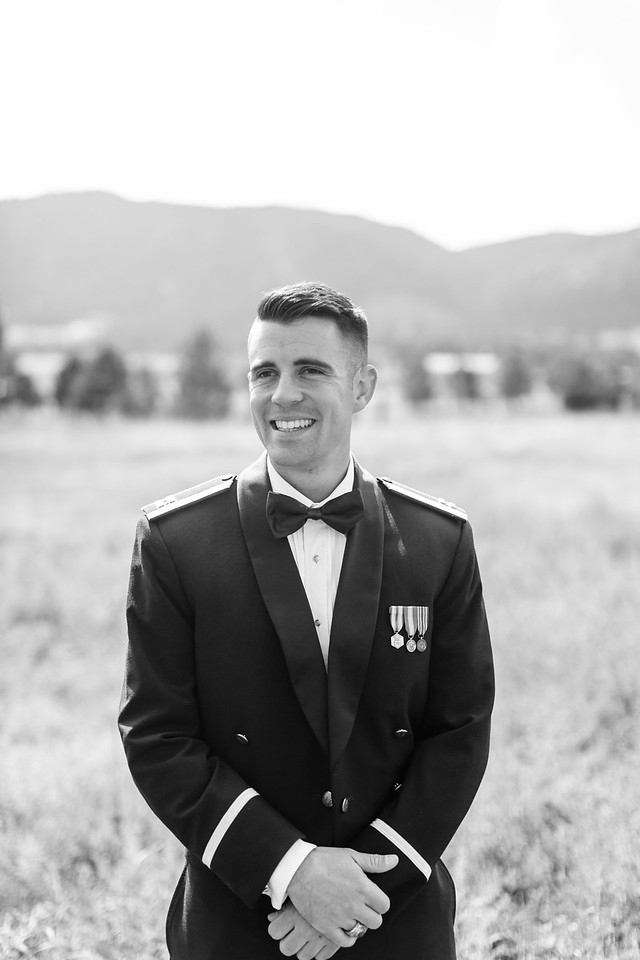
\includegraphics[width=0.4\textwidth]{Kevin.jpg}
\caption{\label{fig:me}Wedding day mess dress (6 Sept 2019).}
\end{figure}

\section{Questions}
\textbf{Question 1- Katrina} What made you interested in data science? 

\textbf{Answer 1:} Great question Katrina! Growing up I was always thinking about doing more things with less time. Whether we were walking to a baseball game, driving around town, buying something, etc I was wanting to do it in an efficient manner (fastest time, cheapest cost). When I was at the USAF Academy, I chose to study Operations Research which analyzes a lot of these same things. I followed up my BS with a MS in OR. When I returned to the USAF Academy, I chose to teach in the Department of Computer and Cyber Sciences and that pushed me to think about the power of computing. OR is very heavy in math and utilizes some programming, but Data Science is quite the opposite. I am interested in Data Science becasue I want to round out my skillset of analyzing problems with a heavier programming skillset.

\paragraph{}
Hey kevin, what are your plans for after the Air Force?  Have you been able to do any on the job research with ML for any Air Force programs?  Good chatting. Talk to you soon.


%\end{document}
